\documentclass[compress]{beamer}
\usepackage{irbookslide}
\usepackage{irilmenau2}
\usepackage{tikz}
\usepackage{url}
\usepackage{ifxetex}
%\RequireXeTeX
\usepackage{fontspec} % zahteva paket euenc
\usepackage{xunicode}
\usepackage{xltxtra}
\usepackage{polyglossia}
\usepackage{minted}
\usepackage{algorithmic}
\renewcommand{\algorithmicrequire}{\textbf{Input:}}
\renewcommand{\algorithmicensure}{\textbf{Output:}}
\usepackage{xcolor,colortbl}
\usepackage{textcomp}
%\setdefaultlanguage[script=Latin]{serbian}

\title{Red sa prioritetom, heap, adaptivni RSP}
\author{\textcopyright \ \ Goodrich, Tamassia, Goldwasser}
\institute{Katedra za informatiku, Fakultet tehničkih nauka, Univerzitet u
Novom Sadu}
\date{2014.}
\subject{Predavanja sa ASP}

\begin{document}

\frame{\titlepage}

\section[Red sa prioritetom]{Red sa prioritetom}
\begin{frame}[fragile]
  \frametitle{Red sa prioritetom}
  \begin{itemize}
    \item \myred{red sa prioritetom} čuva kolekciju elemenata 
    \item svaki element je par (\myred{ključ}, \myred{vrednost})
    \item osnovne operacije:
    \begin{itemize}
      \item \myred{add}($k, x$): dodaje element sa ključem $k$ i vrednošču $x$
      \item \myred{remove\_min}(): uklanja element sa najmanjim ključem 
    \end{itemize}
    \item dodatne operacije:
    \begin{itemize}
      \item \myred{min}(): vraća, ali ne uklanja, element sa najmanjim ključem
      \item \myred{len}(), \myred{is\_empty}() 
    \end{itemize}
  \end{itemize}
\end{frame}

\begin{frame}[fragile,shrink=10]
  \frametitle{Primer operacija nad redom sa prioritetom}
\begin{center}
\begin{tabular}{lcl}
\textbf{operacija} & \textbf{rezultat} & \textbf{sadržaj reda} \\
\hline \hline
\texttt{P.add(5, A)} & -- & [(5,A)] \\ 
\texttt{P.add(9, C)} & -- & [(5,A), (9,C)] \\ 
\texttt{P.add(3, B)} & -- & [(3,B), (5,A), (9,C)] \\ 
\texttt{P.add(7, D)} & -- & [(3,B), (5,A), (7,D), (9,C)] \\ 
\texttt{P.min()} & (3,B) & [(3,B), (5,A), (7,D), (9,C)] \\ 
\texttt{P.remove\_min()} & (3,B) & [(5,A), (7,D), (9,C)] \\ 
\texttt{P.remove\_min()} & (5,A) & [(7,D), (9,C)] \\ 
\texttt{len(P)} & 2 & [(7,D), (9,C)] \\
\texttt{P.remove\_min()} & (7,D) & [(9,C)] \\ 
\texttt{P.remove\_min()} & (9,C) & [ ] \\ 
\texttt{P.is\_empty()} & True & [ ] \\ 
\texttt{P.remove\_min()} & greška & [ ]
\end{tabular}
\end{center}
\end{frame}

\begin{frame}[fragile]
  \frametitle{Ključevi i relacija poretka}
  \begin{itemize}
    \item ključevi mogu biti bilo kog tipa za koga je definisana relacija poretka
    \item elementi u redu mogu imati jednake ključeve -- u tom slučaju se primenjuje FIFO princip
    \item relacija poretka
    \begin{itemize}
      \item refleksivna: $x\leq x$
      \item antisimetrična: $x\leq y \land y\leq x \, \Rightarrow \, x = y$
      \item tranzitivna: $x\leq y \land y\leq z \, \Rightarrow \, x\leq z$
    \end{itemize}
  \end{itemize}
\end{frame}

\begin{frame}[fragile,shrink]
  \frametitle{Element RSP}
\begin{minted}[linenos=false]{python}
class PriorityQueueItem:
  def __init__(self, k, v):
    self.key = k
    self.value = v
    
  def __lt__(self, other):
    return self.key < other.key
    
  def __le__(self, other):
    return self.key <= other.key
\end{minted}
\end{frame}

\begin{frame}[fragile]
\frametitle{Implementacija RSP}
\begin{columns}
  \begin{column}[c]{5.5cm}
    \begin{itemize}
      \item implementacija sa \textbf{nesortiranom} listom
      \item \myred{add} je $O(1)$ jer dodavanje možemo raditi na bilo kom kraju liste
      \item \myred{remove\_min} i \myred{min} su $O(n)$ jer moramo tražiti najmanji ključ u listi
    \end{itemize}
    \begin{center}
      
\includegraphics[width=5cm]{asp-09-pic01a.png}
    \end{center}
  \end{column}
  \begin{column}[c]{5.5cm}
    \begin{itemize}
      \item implementacija sa \textbf{sortiranom} listom
      \item \myred{add} je $O(n)$ jer moramo da nađemo pravo mesto za ubacivanje novog elementa
      \item \myred{remove\_min} i \myred{min} su $O(1)$ jer je najmanji ključ uvek na početku
    \end{itemize}
    \begin{center}
      
\includegraphics[width=5cm]{asp-09-pic01b.png}
    \end{center}
  \end{column}
\end{columns}
\end{frame}

\begin{frame}[fragile,shrink]
  \frametitle{RSP sa nesortiranom listom}
\begin{minted}[linenos=false]{python}
class UnsortedPriorityQueue:
  def __init__(self):
    self._data = SingleList()
    
  def add(self, key, value):
    newest = PriorityQueueItem(key, value) 
    self._data.add_last(newest)
    
  def _find_min(self)
    if self.is_empty():
      raise Empty('Queue is empty')
    smallest = self._data.first()
    current = smallest.next
    while current is not None:
      if current.element < smallest.element:
        smallest = curr
      current = current.next
    return smallest
  
  def remove_min(self):
    p = self._find_min()
    item = self._data.delete(p)
    return (item.key, item.value)
\end{minted}
\end{frame}

\begin{frame}[fragile,shrink]
  \frametitle{RSP sa sortiranom listom}
\begin{minted}[linenos=false]{python}
class SortedPriorityQueue:
  def __init__(self):
    self._data = SingleList()
    
  def add(self, key, value):
    newest = PriorityQueueItem(key, value)
    current = self._data.first()
    while current is not None and newest < current.element:
      current = current.next 
    if current is None:
      self._data.add_first(newest)
    else:
      self._data.add_after(current, newest)
    
  def remove_min(self):
    if self.is_empty():
      raise Empty('Queue is empty')
    item = self._data.delete(self._data.first())
    return (item.key, item.value)
\end{minted}
\end{frame}

\section[Heap]{Heap}
\begin{frame}[fragile]
  \frametitle{Heap}
  \begin{itemize}
    \item \myred{heap} je binarno stablo\ldots 
    \item \ldots čiji elementi su uređeni parovi (\myred{ključ}, \myred{vrednost})
    \item \ldots i koje zadovoljava još 2 uslova:
    \begin{itemize}
      \item \textbf{redosled}: za svaki čvor $n$ osim korena ključ od $n$ je veći ili jednak ključu roditelja od $n$
      \item \textbf{kompletnost}: heap visine $h$ ima nivoe $0, 1, 2,\ldots h-1$ sa maksimalnim brojem čvorova ($i$-ti nivo ima $2^i$ čvorova za $0\leq i\leq
      h-1$)
    \end{itemize}
  \end{itemize}
  \begin{center}
    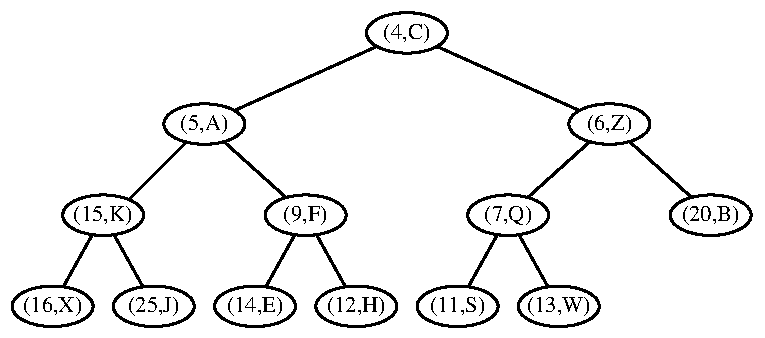
\includegraphics[width=8.5cm]{asp-09-pic02.pdf}
  \end{center}
\end{frame}

\end{document}
